\svnid{$Id$}
\appendix
\chapter{Appendix}
\section{Adaptive step sizes and numerical instability}

\section{\texorpdfstring{Affinity of \cbbthree{} for Oxygen}{Affinity of cbb3 for Oxygen}}
\begin{figure}[h]
 \centering
 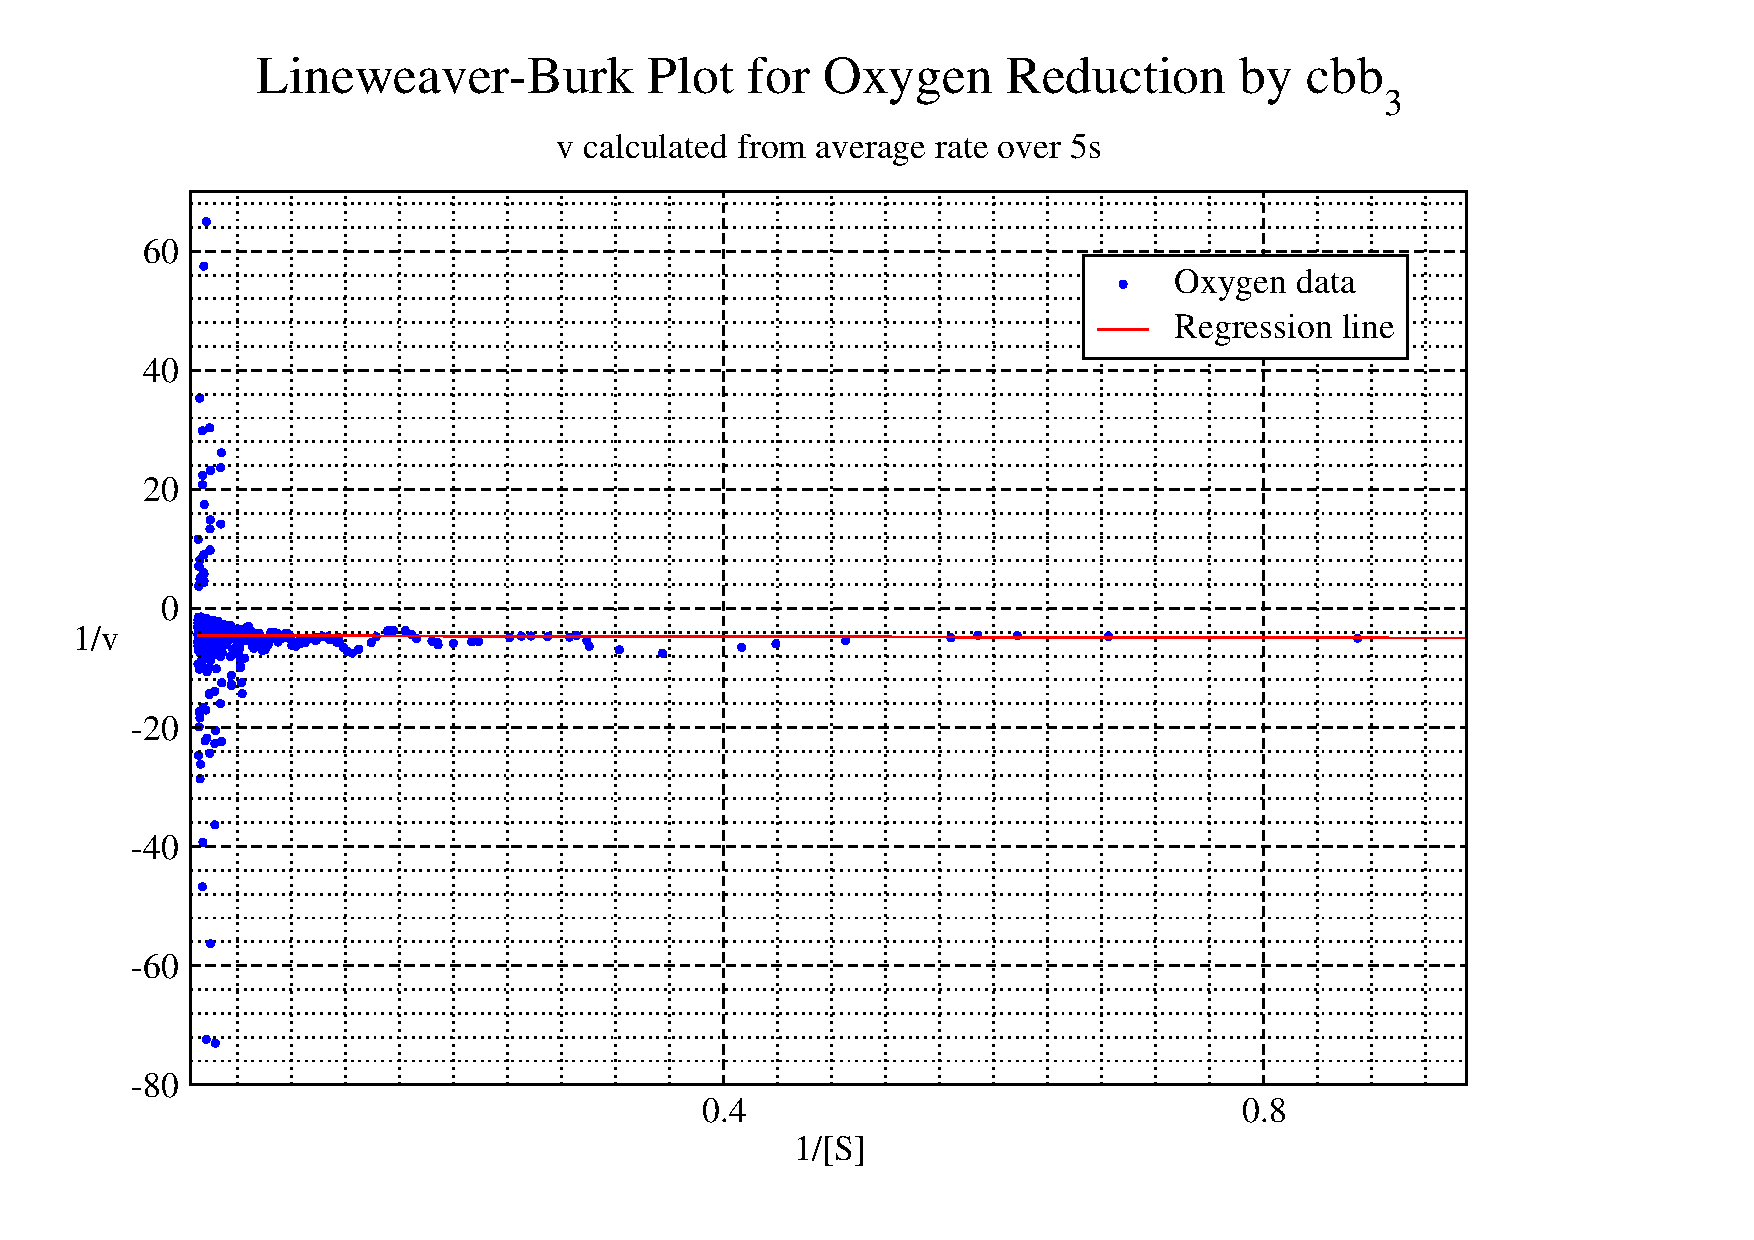
\includegraphics[width=14cm, trim=2cm 1cm 4cm 1cm]{./appendix/data/lbplot.pdf}
 % o2sim.eps: 0x0 pixel, 300dpi, 0.00x0.00 cm, bb=0 0 794 595
 \caption[{Lineweaver-Burk Plot for Oxygen Reduction in \textit{Neisseria meningitidis}.}]{{\bf Lineweaver-Burk Plot for Oxygen Reduction in \textit{Neisseria meningitidis.}} .
 \label{fig:o2lb}}
\end{figure}

\begin{eqnarray}
\frac{d[O_2]}{dt} & = & \beta\left(1-\frac{[O_2]}{K_O}\right) - k_{1}[C_a][O_2] \nonumber \\
\frac{d[NO]}{dt} & = & m_{1}[NO_2^-][A_a] - l_1[NO][B_a] - k_5[C_a][NO] + k_6[C_X] - \gamma[NO] \nonumber \\
\frac{d[NO_2^-]}{dt} & = & - m_{1}[NO_2^-][A_a] \nonumber \\
\frac{d[Q_a]}{dt} & = & g([Q] - [Q_a]) - l_3[Q_a]([B] - [B_a]) - f[Q_a]([X]-[X_a])\ \nonumber \\
\frac{d[X_a]}{dt} & = & -k_3([C] - [C_a] - [C_X])[X_a] - m_3([A] - [A_a])[X_a] + f[Q_a]([X]-[X_a]) \nonumber \\
\frac{d[A_a]}{dt} & = & m_3([A] - [A_a])[X_a] - m_{1}[NO_2^-][A_a] \nonumber \\
\frac{d[B_a]}{dt} & = & l_3[Q_a]([B] - [B_a]) - l_1[NO][B_a] \nonumber \\
\frac{d[C_a]}{dt} & = & k_3([C] - [C_a] - [C_X])[X_a] - k_{1}[C_a][O_2] - k_{5}[C_a][NO] \nonumber \\
\frac{d[C_X]}{dt} & = & k_5[C_a][NO] - k_6 [C_X] \nonumber \\
\frac{d[A]}{dt} & = & \left(R\left(1 - \frac{[O_2] + k_{10}[NO]}{[O_2] + k_{10}[NO] + k_{11}}\right) - S\left(1 - \frac{[NO]}{[NO] + k_{13}}\right)\right) - k_8[A] \nonumber \\
\frac{d[B]}{dt} & = & T \left(\frac{[NO]}{[NO] + k_{15}}\right) - k_{16}[B]
\end{eqnarray}

\begin{table}[ht]
\begin{center}
\begin{tabular}{lcc}
\toprule
\textbf{Symbol} & & \textbf{Description}\\
\midrule
$O_2$ & & Oxygen concentration\\
$NO$ & & Nitric oxide concentration\\
$NO_2^-$ & & Nitrite concentration\\
$X_a$ & & Reduced cytochrome concentration\\
$A_a$& & Reduced AniA\\
$B_a$& & Reduced NorB\\
$C_a$& & Reduced \cbbthree{}\\
$C_X$& & Reversibly inhibited \cbbthree{}\\
$Q_a$& & Reduced Quinones\\
\bottomrule
\end{tabular}
\caption{Model Variables
\label{vs}}
\end{center}
\end{table}



\begin{table}[ht]
\begin{center}
\begin{tabular}{l c}
\toprule
\textbf{Symbol} & \textbf{Description}\\
\midrule
$k_1$ & Rate constant for O$_{\textrm{2}}$ reduction by reduced \cbbthree{}\\
$k_3$ & Rate constant for \cbbthree{} reduction by cytochrome pool\\
$l_1$ & Rate constant for NO reduction by reduced NorB\\
$l_3$ & Rate constant for NorB reduction by quinone pool\\
$m_1$ & Rate constant for NO$_{\textrm{2}}^{\textrm{-}}$ reduction by reduced AniA\\
$m_3$ & Rate constant for AniA reduction by cytochrome pool\\
$k_5$ & Rate constant for \cbbthree{} inhibition by NO\\
$k_6$ & Rate constant for recovery of NO inhibited \cbbthree{}\\
$\beta$ & Rate constant for passive diffusion in of O$_{\textrm{2}}$\\
$K_O$ & Saturation O$_{\textrm{2}}$ level\\
$g$ & Rate of electrons in from NADH\\
$f$ & Rate constant for reduction of cytochromes by quinones\\
$\gamma$ & Spontaneous loss of NO\\
$Q$ & Concentration of quinones\\
$X$ & Concentration of cytochromes\\
$A$ & Concentration of AniA\\
$B$ & Concentration of NorB\\
$C$ & Concentration of \cbbthree{}\\
\bottomrule
\end{tabular}
\caption{Model Parameters
\label{ps}}
\end{center}
\end{table}